

\subsection{Соединения галогенов в степени окисления (-1), межгалогенные соединения, способы получения, химическое поведение, электронное и геометрическое строение молекул.}

\subsubsection*{Галогенводороды}

\textbf{Получение}

1) Прямой синтез из элементов

$$H_2 + X_2 = 2HX$$
($F_2, Cl_2$ -со взрывом, $Br_2, I_2$ - спокойнее, т.к. равновесие смещено влево)

2) Вытеснение HX из солей

$$CaF_{2(tv)} + H_2SO_{4(konc)} \rightarrow CaSO_4\downarrow + 2HF\uparrow$$
$$NaCl + H_2SO_{4(konc)} \rightarrow NaHSO_4 + HCl\uparrow$$
$$KX + H_3PO_{4(konc)} \rightarrow KH_2PO_4 + HX\uparrow$$

3) Гидролиз галогенидов неметаллов

$$SiCl_4 + 3H_2O \rightarrow H_2SiO_3 + 4HCl \uparrow$$
$$PX3 + 3H_2O  \rightarrow H_3PO_4 + 3HX\uparrow$$
$$2P_{kr} + 3X_2 + 6H_2O \rightarrow 2H_3PO_4 + 6HX$$

4) Галогенирование углеводородов

Побочные продукты при хлорировании и бромировании алканов и циклоалканов

5) Концентрированные кислоты

$$3Br_2 + S + 4H_2O \rightarrow H_2SO_4 + 6HBr$$
$$H_2S + I_2 \rightarrow 2HI + S\downarrow$$

\textbf{Химические свойства}

1) Кислоты в водных растворах

$$HX + HOH \rightleftharpoons X^- + H_3O^+$$
HF - слабая, HCl, HBr, HI - сильные, увеличение силы кислот

2) Восстановители (кроме HF)

$$MnO_{2(tv)} + 4HCl_{konc} \rightarrow MnCl_2 + 2H_2O + Cl_2$$

$$2HI + 2FeCl_3 \rightarrow 2FeCl_2 + I_2 + 2HCl$$

$$4HI + 2CuSO_4 \rightarrow2CuI\downarrow + I_2 + 2H_2SO_4$$

3) Азеотропные смеси с водой
 
4) Особые свойства HF

а) Водородные  связи

б) Образование гидрофторидов

$$HF + F^- \rightarrow HF_2^-$$
$[F-H-F]^-$ - линейный

в) с $SiO_2$

$$4HF{gas} + SiO_2 \rightarrow SiF_4\uparrow + 2H_2O$$

\textbf{Электронное и геометрическое строение молекул}

Линейные полярные молекулы

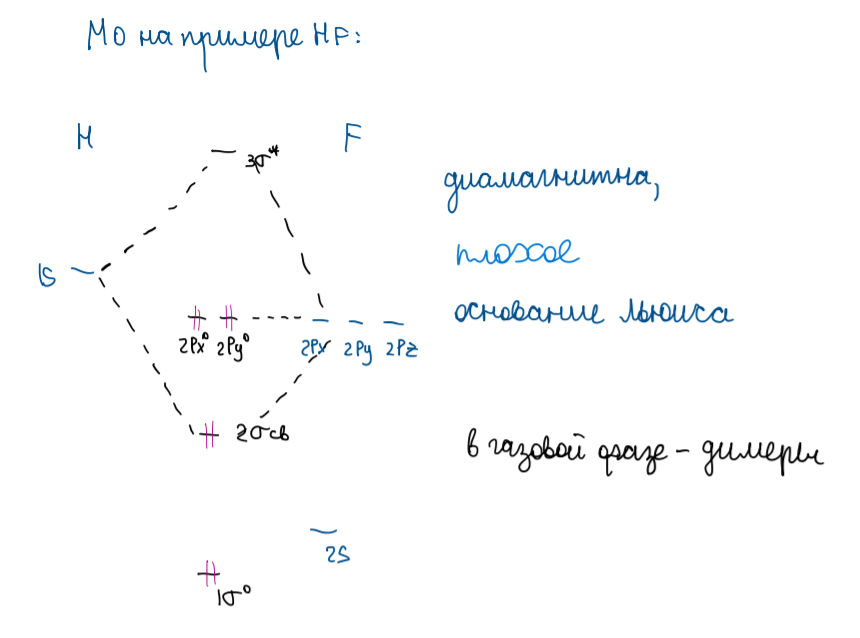
\includegraphics{images/4v1.png}

\subsubsection*{Галогениды}

\textbf{Способы получения}

1) Обменные реакции солей

2) Металлы (до Сг) c HX

$$Me + HX \rightarrow MeX_n + H_2\uparrow$$

3) Прямое воздействие металла с $X_2$

$$2Sb + 3I_2 \rightarrow 2SbI_3 (C_6H_6)$$

4) Галогенирование оксидов с помощью $Cl_2(Br_2)$ в присутствии угля

$$Ta_2O_5 + 5C + 5Br_2 \rightarrow 2TaBr_5 +5CO \uparrow$$

(галогенирующими веществами могут быть $NH_4Cl, CCl_4, CoCl_2, ClF_3$)

5) Дегидратация кристаллогидратов

$$NiCl_2\cdot6H_2O + 6SOCl_2 \rightarrow NiCl_2 + 6SO_2\uparrow + 12HCl\uparrow$$

\textbf{{Химические свойства}}

1) Обменные реакции с солями
2) Гидролиз
$$PCl_5 + 4H_2O \rightarrow 5HCl + H_3PO_4$$
3) Восстановители

$$MeI_2 + H_2SO_{4(konc)} \rightarrow I_2 + H_2S + MeSO4 + H_2O$$
$$MeBr_2 + H_2SO_{3(konc)} \rightarrow Br_2 + SO_2 + MeSO_4 + H_2O$$

\textbf{Электронное и геометрическое строение молекул}

1) Ионные (Щ, Щ/М, РЗ металлы)

$NaCl$ - ГЦК, кч=6\\
$CsCl$ - ОЦК, кч = 8\\
$CaF_2$ - КЧ($Ca^{2+}$) =8; кч($F^-$) =4

2) Ковалентные

d-Me в низких с.о., p-Me с низкой эо.

3) Молекулярные

p-Me с высокой эо, d-Me в высших с.о.

\subsubsection*{Межгалогенные соединения}

\textbf{Способы получения}

1) Непосредственное взамодействие простых веществ при варьировании соотношения реагентов, температуры и давления

2) Из сложных веществ галогенирующими агентами

$$KI + 4F_2 \rightarrow KF_{tv} + IF_7 (250^{\circ})$$

3) Галогенирование низших галогенидов

$$ClF_3 + F_2 \rightarrow ClF_5$$

\textbf{Химические свойства}

1) С $H_2O$

a) Гидролиз
$$BrF_5 + 3H_2O \rightarrow HBr_O3 + 5HF$$

б) Диспропорционирование

$$5ICl_3 + 9H_2O \rightarrow I_2 + 3HIO_3 + 15HCl$$

2) В качестве галогенирующих агентов

$$W + 6ClF \rightarrow WF_6 + 3Cl_2$$
$$2Co_3O_4 + 6ClF_3 \rightarrow 6CoF_3 + 3Cl_2 + 4O_2$$

3) Кислотно-основные свойства

$$BrF_3 + CsF \rightarrow CsBrF_4$$
$$BrF_3 + SbF_5 \rightarrow [BrF_2]^+[SbF_6]^-$$

4) С растворами щелочей до соответствующих солей: 

$$IF_5 + 6NaOH \rightarrow 5NaF + NaIO_3 + 3H_2O$$

\textbf{Электронное и геометрическое строение}

Все молекулы диамагнитны\\
Строение описывается на основе метода Гиллеспи

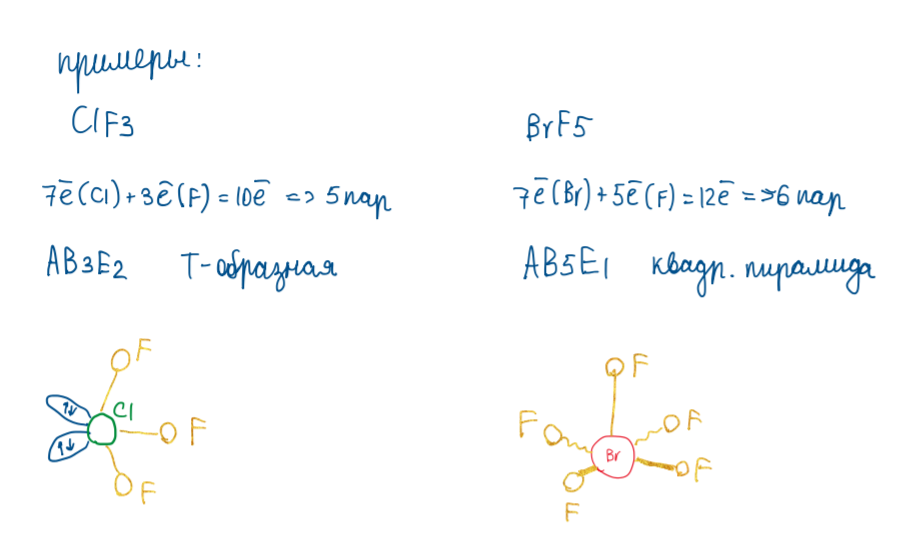
\includegraphics{images/4v2.png}